\begin{figure}[b!]
  \vspace{-2em}
  \centering
  \subfloat[True QoI.]{
    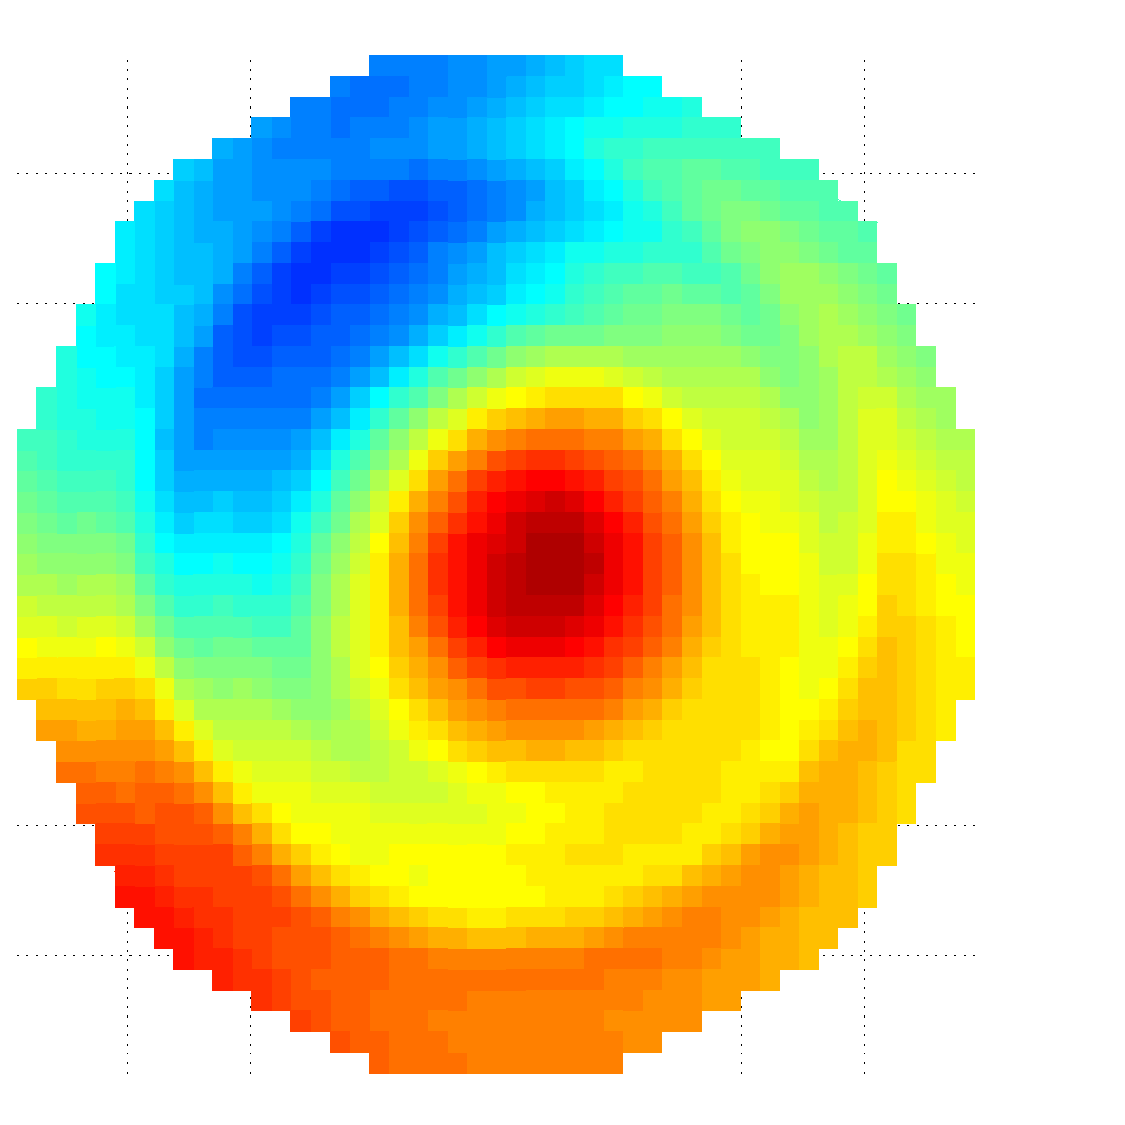
\includegraphics[width=0.4\linewidth]{include/assets/wafer-qoi-true.pdf}
    \flabel{wafer-qoi-true}
  }
  \subfloat[Inferred QoI.]{
    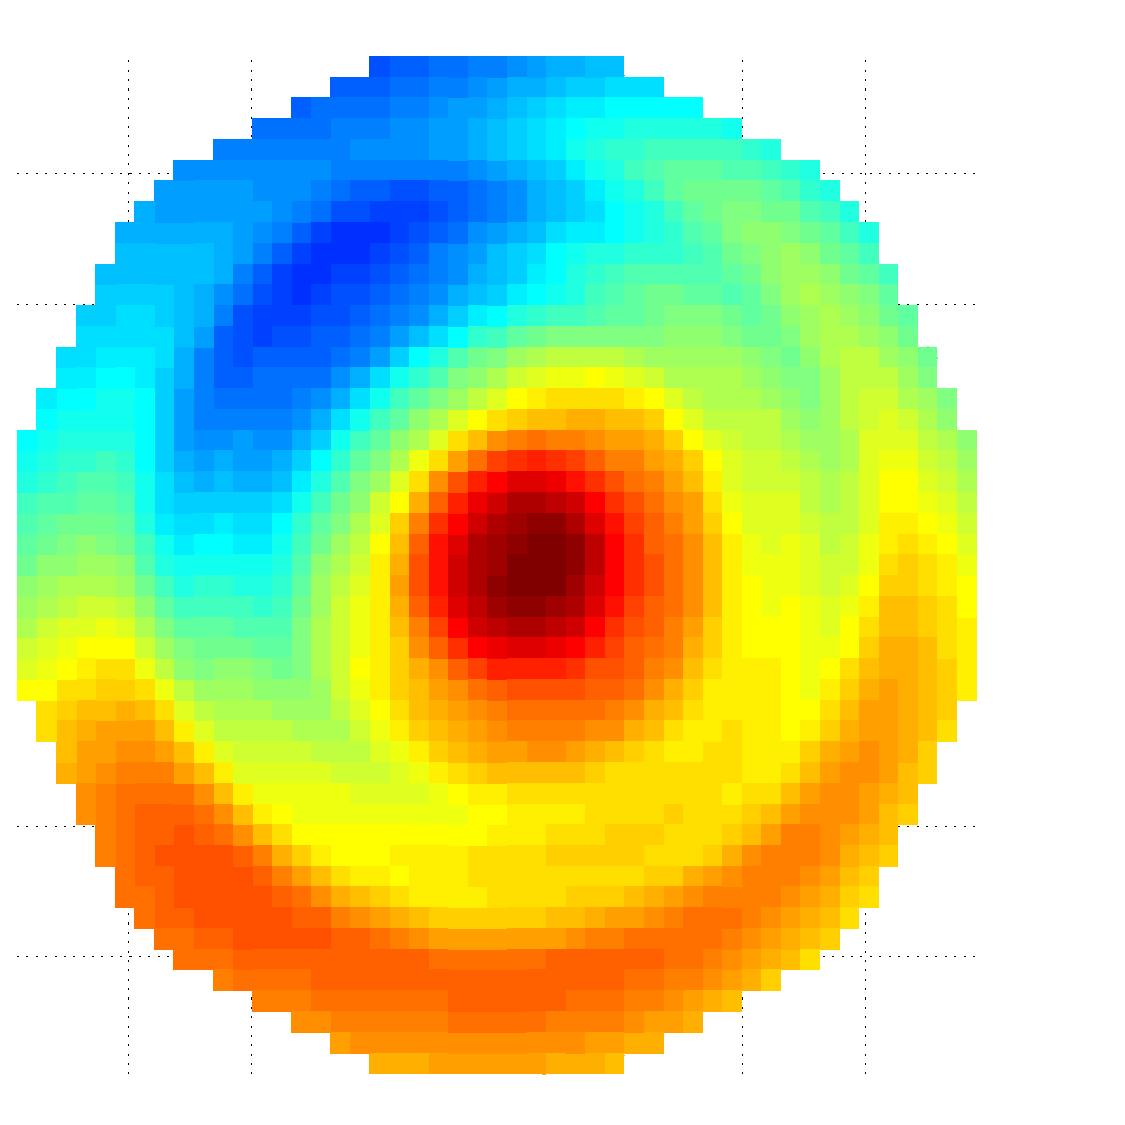
\includegraphics[width=0.4\linewidth]{include/assets/wafer-qoi-inferred.pdf}
    \flabel{wafer-qoi-inferred}
  }
  \caption{The distribution of the QoI across the wafer.}
\end{figure}

Let us consider an important application of the proposed technique: the characterization of the distribution, across the wafer, of the effective channel length, denoted by $\u$. The effective channel length has one of the strongest effects on the subthreshold leakage current and, consequently, on power and temperature \cite{juan2011, juan2012}; at the same time, $\u$ is well-known to be severely deteriorated by process variation \cite{chandrakasan2001, srivastava2010}.
Assume the technological process imposes a lower bound $\u_*$ on $\u$. This bound separates defective dies ($\u < \u_*$) from those that function properly ($\u \geq \u_*$).
In order to reduce costs, the manufacturer is interested in detecting the faulty dies and taking them out of the production process at early stages. Then, the possible actions that they might take with respect to a single die on the wafer are: (a) keep the die if it closely conforms to the specification; (b) recycle the die, otherwise.
Let the distribution of the effective channel length across the wafer be the one depicted on the left side of \fref{wafer-qoi} where the gradient from navy to dark red represents the transition of $\u$ from low to high values (the experimental setup will be described in detail in \sref{experimental-results}); hence, the navy regions are the areas with a high level of the power/temperature dissipation.
One way to find this distribution is to perform intrusive measurements by destroying the dies and taking samples of $\u$ directly. Another solution is to restrain our ambitions and change the \qoi\ to some other parameter, which can be measured without the need of damaging the dies, \eg, to the leakage current. In either way, one has to deploy adequate test structures on the dies and perform the measurements of the \qoi\ directly. The problem, however, is that the described procedure is technologically complex and, thus, might significantly increase the production costs. Furthermore, the first solution implies that all the measured dies have to be thrown away afterwards, and the second implies that the further design decisions will be based on a surrogate quantity instead of the primary source of uncertainty, \ie, the effective channel length, which can compromise the reliability of such decisions.

The technique developed in this paper works differently. We apply a fixed workload to a small number of dies on the wafer and measure the corresponding temperature profiles. These profiles can be potentially corrupted by the measurement noise. Since temperature is cheap to track using, \eg, infrared cameras and no on-die test structures are required, our approach can considerably decrease the costs associated with the characterization of process variation and further decision making.
The result of our framework applied to a data set---wherein only 20 out of 316 dies on the wafer, marked with crosses in \fref{wafer-measured}---have been measured, is shown on the right side of \fref{wafer-qoi}. It can be seen that the two distributions closely match each other. Hence, based on less than $7\%$ of the dies, we can characterize the effective channel length with a high level of accuracy.

Another feature of the proposed framework is that probabilities of various events, \eg, $\probabilityMeasure(\u \geq \u_*)$, can readily be estimated.
This is important since, in reality, the true values of the \qoi\ remain unknown to us (otherwise, we would not need to quantify them), and, therefore, we can rely on our decisions only up to a certain probability.
We can then reformulate the decision rule defined earlier as follows: (a) keep the die if $\probabilityMeasure(\u \geq \u_*)$ is larger than a certain threshold; (b) recycle the die, otherwise.
An illustration of this rule is given in \fref{wafer-defective} where the lower bound $\u_*$ is set to two standard deviations below the mean value of the effective channel length; the probability threshold of the action (a) is set to 0.9; the crosses mark both the true and inferred defective dies (they coincide); and the gradient from light gray to red corresponds to the inferred probability of a die to be defective. It can be seen that the inference accurately detects faulty regions.
\begin{figure}
  \centering
  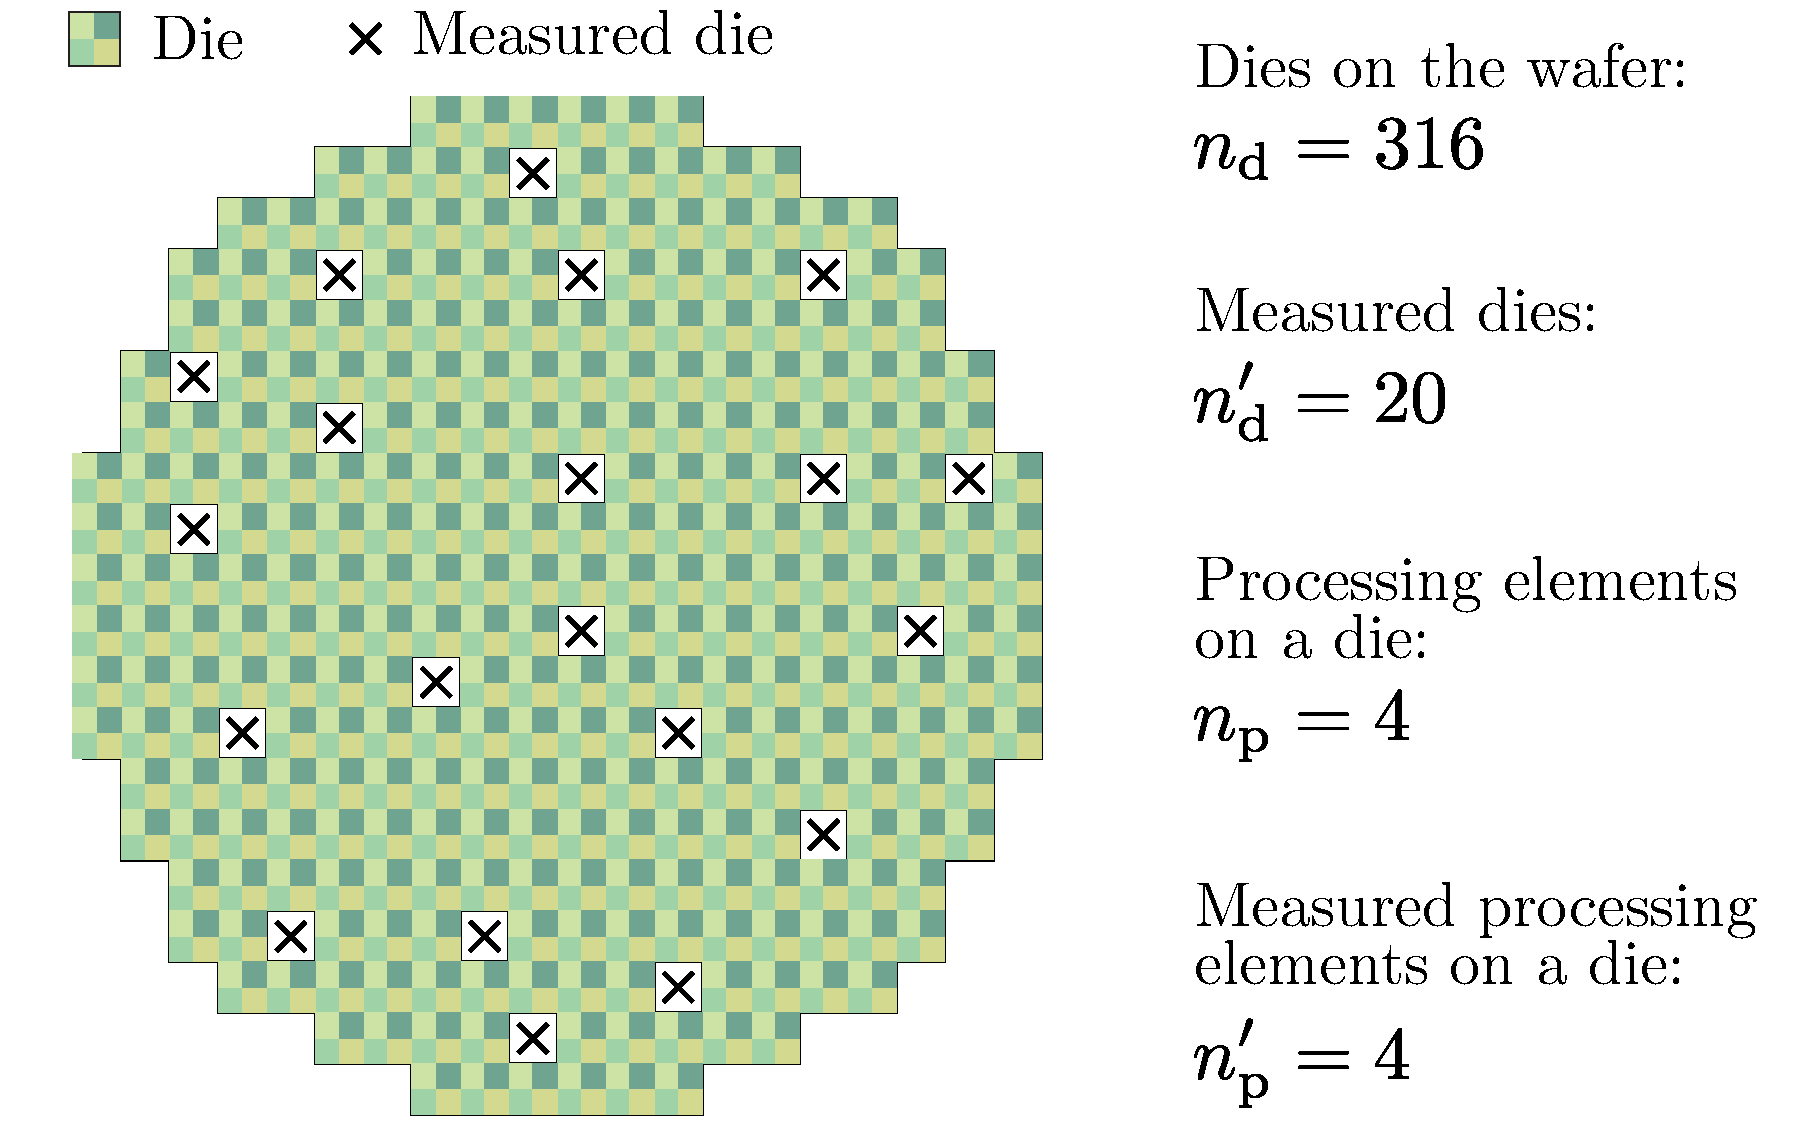
\includegraphics[width=0.9\linewidth]{include/figures/wafer-measured.pdf}
  \caption{Measured dies on the wafer.}
  \flabel{wafer-measured}
  \vspace{-1.5em}
\end{figure}

\begin{figure}[b]
  \vspace{-1.5em}
  \centering
  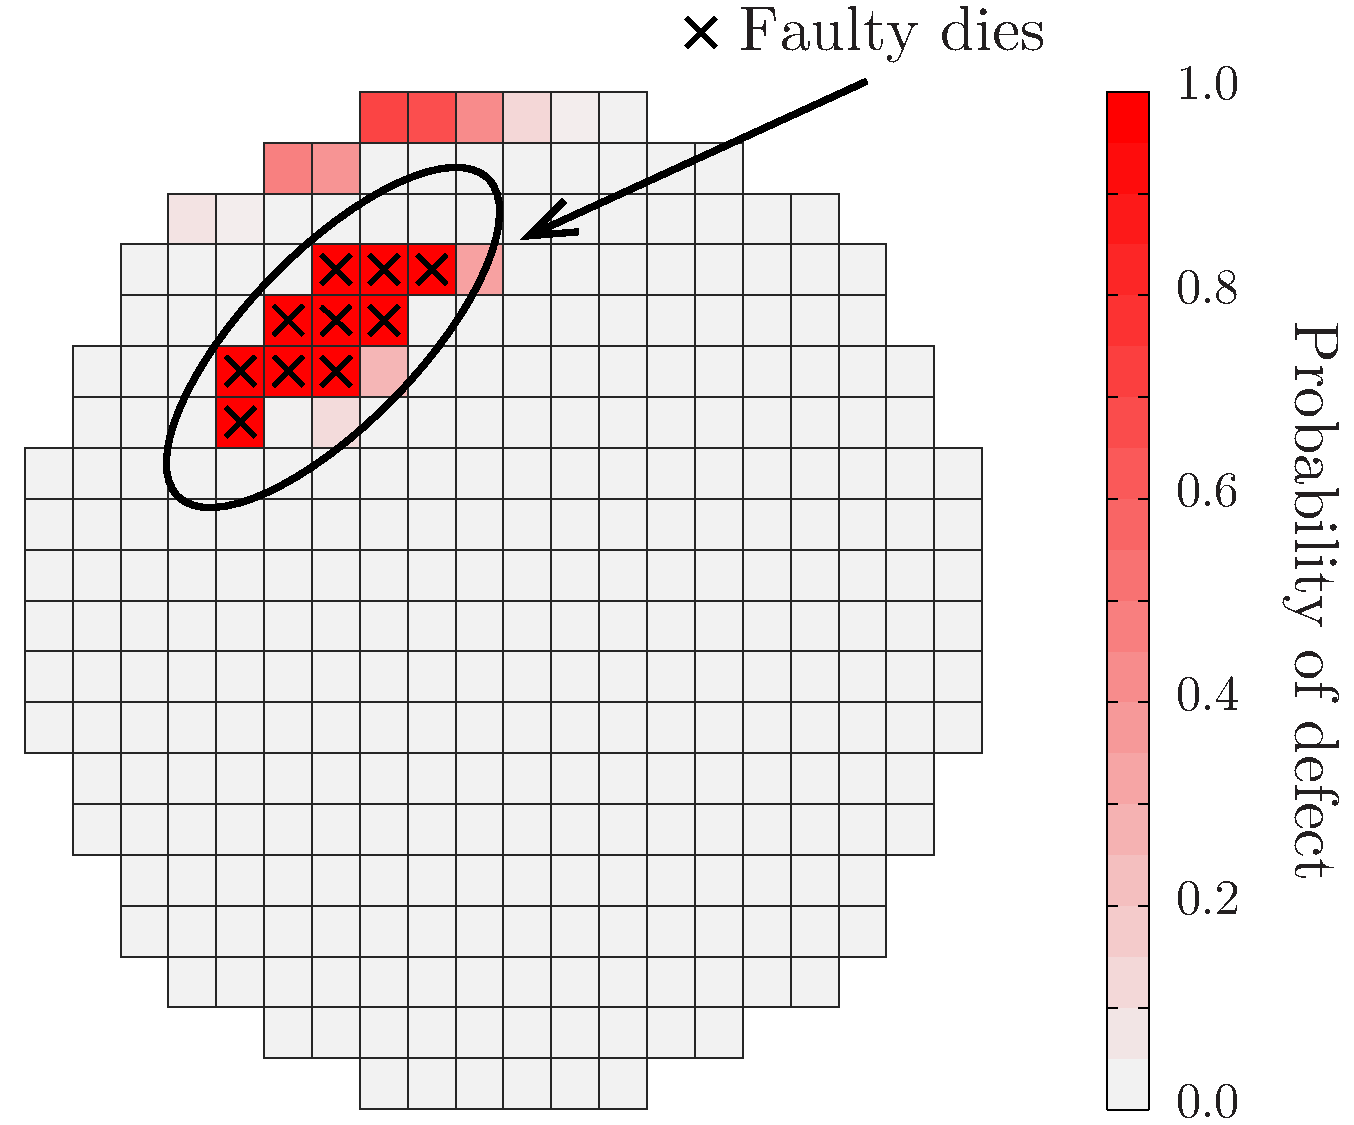
\includegraphics[width=0.9\linewidth]{include/figures/wafer-defective.pdf}
  \caption{Inferred probability of defect.}
  \flabel{wafer-defective}
\end{figure}


In addition, we can introduce a trade-off action: (c) expose the die to a thorough inspection (\eg, via a test structure) if $\probabilityMeasure(\u \geq \u_*)$ is smaller than the threshold of (a) and is larger than some other threshold, \eg, $0.1 < \probabilityMeasure(\u \geq \u_*) < 0.9$. In this case, we can reduce costs by examining only those dies for which there is neither sufficiently strong evidence of their satisfactory nor unsatisfactory condition.
Furthermore, one can introduce in the inference a so-called utility function, which, for each combination of an outcome of the effective channel length and a taken action, returns the corresponding gain that the decision maker obtains.
For example, such a utility function can encode that an excessive inspection, action (c), which would confirm the correctness of the die, costs more than an incorrectly discarded die.
The optimal decision is given by the action that maximizes the expected utility with respect to both the observed data and the prior knowledge on $\u$ \cite{bernardo2007}.
In other words, all possible outcomes of the effective channel length weighted by their probabilities will be taken into account in the final decision, also incorporating the preferences of the user via the utility function.
